% vim: set ts=4 sw=4 tw=80 noexpandtab:

\documentclass{42-en}

%******************************************************************************%
%                                                                              %
%                                   Prologue                                   %
%                                                                              %
%******************************************************************************%
\usepackage[
    type={CC},
    modifier={by-nc-sa},
    version={4.0},
]{doclicense}
\usepackage{amsmath} % The amsmath package provides commands to typeset matrices with different delimiters. 
\usepackage{epigraph}
\setlength\epigraphwidth{.95\textwidth}
%****************************************************************%
%                  Re/definition of commands                     %
%****************************************************************%

\newcommand{\ailogo}[1]{\def \@ailogo {#1}}\ailogo{assets/42ai_logo.pdf}

%%  Redefine \maketitle
\makeatletter
\def \maketitle {
  \begin{titlepage}
    \begin{center}
	%\begin{figure}[t]
	  %\includegraphics[height=8cm]{\@ailogo}
	  
\includegraphics[height=8cm]{assets/42ai_logo.pdf}
	%\end{figure}
      \vskip 5em
      {\huge \@title}
      \vskip 2em
      {\LARGE \@subtitle}
      \vskip 4em
    \end{center}
    %\begin{center}
	  %\@author
    %\end{center}
	%\vskip 5em
  \vfill
  \begin{center}
    \emph{\summarytitle : \@summary}
  \end{center}
  \vspace{2cm}
  %\vskip 5em
  %\doclicenseThis
  \end{titlepage}
}
\makeatother

\makeatletter
\def \makeheaderfilesforbidden
{
  \noindent
  \begin{tabularx}{\textwidth}{|X X  X X|}
    \hline
  \multicolumn{1}{|>{\raggedright}m{1cm}|}
  {\vskip 2mm 
\includegraphics[height=1cm]{assets/42ai_logo.pdf}} &
  \multicolumn{2}{>{\centering}m{12cm}}{\small Exercise : \@exnumber } &
  \multicolumn{1}{ >{\raggedleft}p{1.5cm}|}
%%              {\scriptsize points : \@exscore} \\ \hline
              {} \\ \hline

  \multicolumn{4}{|>{\centering}m{15cm}|}
              {\small \@extitle} \\ \hline

  \multicolumn{4}{|>{\raggedright}m{15cm}|}
              {\small Turn-in directory : \ttfamily
                $ex\@exnumber/$ }
              \\ \hline
  \multicolumn{4}{|>{\raggedright}m{15cm}|}
              {\small Files to turn in : \ttfamily \@exfiles }
              \\ \hline

  \multicolumn{4}{|>{\raggedright}m{15cm}|}
              {\small Forbidden functions : \ttfamily \@exforbidden }
              \\ \hline

%%  \multicolumn{4}{|>{\raggedright}m{15cm}|}
%%              {\small Remarks : \ttfamily \@exnotes }
%%              \\ \hline
\end{tabularx}
%% \exnotes
\exrules
\exmake
\exauthorize{None}
\exforbidden{None}
\extitle{}
\exnumber{}
}
\makeatother

%%  Syntactic highlights
\makeatletter
\newenvironment{pythoncode}{%
  \VerbatimEnvironment
  \usemintedstyle{emacs}
  \minted@resetoptions
  \setkeys{minted@opt}{bgcolor=black,formatcom=\color{lightgrey},fontsize=\scriptsize}
  \begin{figure}[ht!]
    \centering
    \begin{minipage}{16cm}
      \begin{VerbatimOut}{\jobname.pyg}}
{%[
      \end{VerbatimOut}
      \minted@pygmentize{c}
      \DeleteFile{\jobname.pyg}
    \end{minipage}
\end{figure}}
\makeatother

\usemintedstyle{native}

\begin{document}

% =============================================================================%
%                     =====================================                    %

\title{Machine Learning - Module 02}
\subtitle{Multivariate Linear Regression}
\author{
  Maxime Choulika (cmaxime), Pierre Peigné (ppeigne), Matthieu David (mdavid)
}

\summary
{
  Building on what you did on the previous modules you will extend the linear regression to handle more than one features.
  Then you will see how to build polynomial models and how to detect overfitting.
}

\maketitle
%******************************************************************************%
%                                                                              %
%                        Section usefull ressources                            %
%                          for ML Modules                                      %
%                                                                              %
%******************************************************************************%


\chapter*{Notions and ressources}

\section*{Notions of the module}
Regularization, overfitting. Regularized loss function, regularized gradient descent.  
Regularized linear regression. Regularized logistic regression.

\section*{Useful Ressources}

You are strongly advise to use the following resource:
\href{https://www.coursera.org/learn/machine-learning}{Machine Learning MOOC - Stanford}
These videos are available at no cost; simply log in, select "Enroll for Free", and choose "audit the course for free" in the popup window.
The following sections of the course are pertinent to today's exercises:

\newpage

\subsection*{Week 3: Classification}

\subsubsection*{Classification with logistic regression (already seen on module 03)}
\begin{itemize}
  \item Motivations
  \item Logistic regression
  \item Decision boundary
\end{itemize}

\subsubsection*{Cost function for logistic regression (already seen on module 03)}
\begin{itemize}
  \item Cost function for logistic regression
  \item Simplified Cost Function for Logistic Regression
\end{itemize}

\subsubsection*{Gradient descent for logistic regression (already seen on module 03)}
\begin{itemize}
  \item Gradient Descent Implementation
\end{itemize}

\subsubsection*{The problem of overfitting (New !!!)}
\begin{itemize}
  \item The problem of overfitting
  \item Addressing overfitting
  \item Cost function with regularization
  \item Regularized linear regression
  \item Regularized logistic regression  
\end{itemize}


\emph{All videos above are available also on this \href{https://youtube.com/playlist?list=PLkDaE6sCZn6FNC6YRfRQc_FbeQrF8BwGI&feature=shared}{Andrew Ng's YouTube playlist}, videos from 31 to 36 (already seen on module 03) and 37 to 41 (new !!!).}
%******************************************************************************%
%                                                                              %
%                        Common Instructions                                   %
%                          for Python Projects                                 %
%                                                                              %
%******************************************************************************%

\chapter*{Common Instructions}
\begin{itemize}
  \item The version of Python recommended to use is 3.7, you can
  check the version of Python with the following command: \texttt{python -V}
  
  \item The norm: during this piscine, it is recommended to follow the
  \href{https://www.python.org/dev/peps/pep-0008/}{PEP 8 standards}, though it is not mandatory.
  You can install \href{https://pypi.org/project/pycodestyle}{pycodestyle} which
  is a tool to check your Python code.
  
  \item The function \texttt{eval} is never allowed.
  
  \item The exercises are ordered from the easiest to the hardest.
  
  \item Your exercises are going to be evaluated by someone else,
  so make sure that your variable names and function names are appropriate and civil. 
  
  \item Your manual is the internet.
  
  \item You can also ask questions on the {https://discord.gg/8Vvb6QMCZq}{42AI} discord.
  
  \item If you find any issue or mistakes in the subject please create an issue on \href{https://github.com/42-AI/bootcamp_python/issues}{42AI repository on Github}.  
  
  \item We encourage you to create test programs for your
  project even though this work \textbf{won't have to be
  submitted and won't be graded}. It will give you a chance
  to easily test your work and your peers’ work. You will find
  those tests especially useful during your defence. Indeed,
  during defence, you are free to use your tests and/or the
  tests of the peer you are evaluating.
  
  \item Submit your work to your assigned git repository. Only the work in the
  git repository will be graded. If Deepthought is assigned to grade your
  work, it will be run after your peer-evaluations.
  If an error happens in any section of your work during Deepthought's grading,
  the evaluation will stop.
\end{itemize}

\newpage
\tableofcontents
\startexercices

%                     =====================================                    %
% =============================================================================%


%******************************************************************************%
%                                                                              %
%                                   Exercises                                  %
%                                                                              %
%******************************************************************************%

% ============================================== %
% ===========================(start ex 00)       %
\chapter{Exercise 00}
%******************************************************************************%
%                                                                              %
%                                 Interlude                                    %
%                         for Machine Learning module                          %
%                                                                              %
%******************************************************************************%

% =============================== %
\section*{Interlude}
% =============================== %
\subsection*{Classification: The Art of Labelling Things}
% ******************************* %
Over the last three modules you have implemented your first machine learning algorithm.\\
\\
You are now familiar the three-steps cycle we follow when we build \textbf{learning algorithms}:
\\
\begin{figure}[!h]
    \centering
    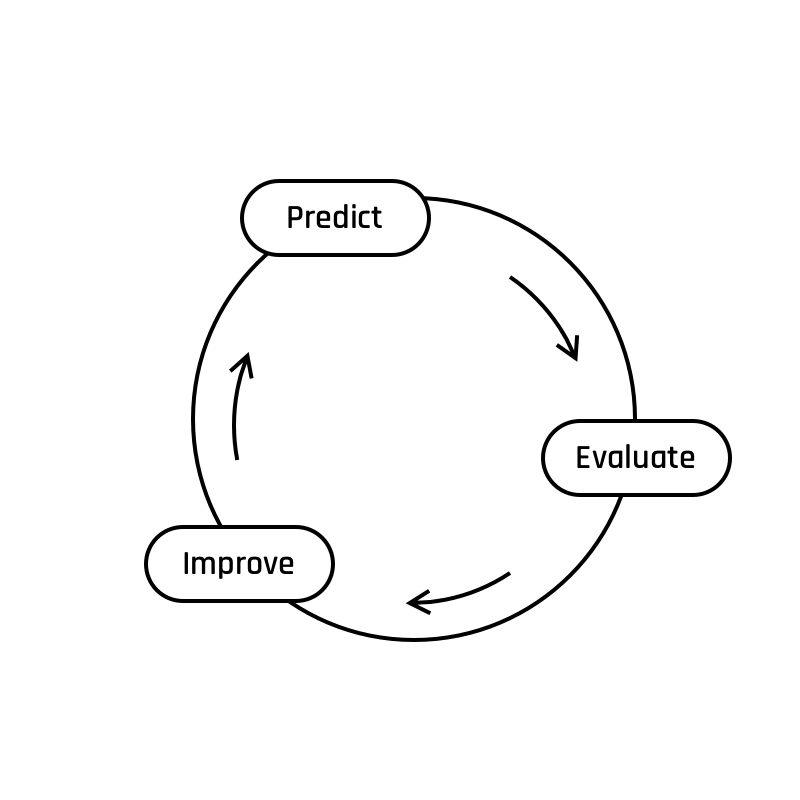
\includegraphics[scale=0.25]{assets/Default.png}
    %\caption{The Learning Cycle}
\end{figure}
\\
The first algorithm you discovered, \textbf{Multivariate Linear Regression}, can now be used to predict a numerical value, based on several features.
This algorithm uses gradient descent to optimize its loss function.\\
\\
Now let's introduce your first \textbf{classification algorithm}: the notorious \textbf{Logistic Regression.}
\hint{regression vs classification; discrete vs continuous values}
\newpage
\noindent{\textbf{Logistic regression} performs a \textit{classification task}, which means that you are not predicting a numerical value (like price, age, grades...) 
but \textbf{categories}, or \textbf{labels} (like dog, cat, sick/healty...)}.
\\
\warn{
    Don't be confused by the word \textit{'regression'} in \textbf{Logistic Regression}.
    It really is a \textit{classification task}! The name is a bit tricky but you will quickly get used to it.
    Once again: \textbf{Logistic Regression is a classification algorithm} which assigns a label/category/class to a given example.
}
\info{
    In this module we will use the following terms interchangeably: \textbf{class}, \textbf{category}, and \textbf{label}.
    They all refer to the \textit{groups} to which each training example can be assigned to, in a classification task.
}

% =============================== %
\subsection*{Predict I: Introducing the Sigmoid Function}
% ******************************* %

\begin{figure}[!h]
    \centering
    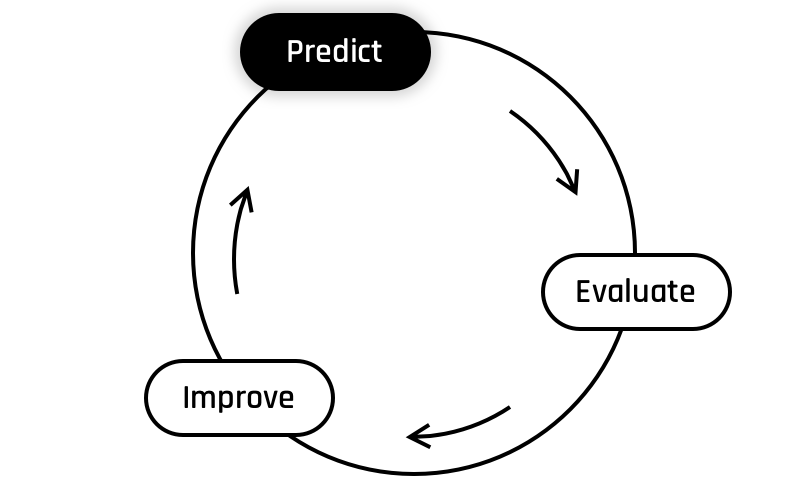
\includegraphics[scale=0.25]{assets/Predict.png}
    %\caption{The Learning Cycle - Predict}
\end{figure}

% =============================== %
\subsubsection*{Formulating a Hypothesis}
% ******************************* %
Remember that a hypothesis, denoted $h(\theta)$, is an equation that combines a set of \textbf{features} (that characterizes an example) with \textbf{parameters} in order to output a \textbf{prediction}.\\
\\
Remember the hypothesis we used in linear regression?\\
$$
h(\theta) = \theta_0 + \theta_{1} x_{1}^{(i)} + \dots + \theta_{n} x_{n}^{(i)} = \theta \cdot x'^{(i)}
$$
\newline
It worked fine to predict continuous values, but could we also use it to tell, for example, 
if a patient is sick or not?
That's a yes-or-no question, so the output from the hypothesis function should reflect that.\\
\\
To get started, we will assign each class a numerical value: sick patients will be 
assigned a value of 1, and healthy patients will be assigned a value of 0.\\
The goal will be to build a hypothesis that outputs a probability that a patient is sick as a float number in the range of [0, 1].\\
\\
The good news is that we can keep the linear equation we already worked with!\\
\\
All we need to do is squash its output through another function that is bounded between 0 and 1.\\
\\
That's the purpose of the \textbf{Sigmoid function} and your next assignment is to implement it!

\newpage
\extitle{Multivariate Hypothesis - Iterative Version}
\turnindir{ex00}
\exnumber{00}
\exfiles{prediction.py}
\exforbidden{None}
\makeheaderfilesforbidden

% ================================== %
\section*{Objective}
% ---------------------------------- %
Manipulate the hypothesis to make prediction.\
You must implement the following formula as a function:

$$
\begin{matrix}
  \hat{y}^{(i)} = \theta_0 + \theta_1 x_{1}^{(i)}  + \dots + \theta_n x_{n}^{(i)} && & \text{ for i = 1, ..., m}
\end{matrix}
$$
  
Where:
\begin{itemize}
  \item $\hat{y}$ is a vector of dimension $m$: the vector of predicted values,
  \item $\hat{y}^{(i)}$ is the i$^\text{th}$ component of the $\hat{y}$ vector: the predicted value for the i$^\text{th}$ example,
  \item $\theta$ is a vector of dimension $(n + 1)$: the parameter vector,
  \item $\theta_j$ is the j$^\text{th}$ component of the parameter vector,
  \item $X$ is a matrix of dimensions $(m \times n)$: the design matrix,
  \item $x^{(i)}$ is the i$^\text{th}$ row of the $X$ matrix: the feature vector of the i$^\text{th}$ example,
  \item $x_{j}$ is the j$^\text{th}$ column of the $X$ matrix,
  \item $x_j^{(i)}$ is the element at the intersection of the i$^\text{th}$ row and the j$^\text{th}$ column of the $X$ matrix: the j$^\text{th}$ feature of the i$^\text{th}$ example
\end{itemize}


% ================================== %
\section*{Instructions}
% ---------------------------------- %

In the \texttt{prediction.py} file, create the following function as per the instructions given below:
\par
\begin{minted}[bgcolor=darcula-back,formatcom=\color{lightgrey},fontsize=\scriptsize]{python}
  def simple_predict(x, theta):
      """Computes the prediction vector y_hat from two non-empty numpy.array.
      Args:
        x: has to be an numpy.array, a matrix of dimension m * n.
        theta: has to be an numpy.array, a vector of dimension (n + 1) * 1.
      Return:
        y_hat as a numpy.array, a vector of dimension m * 1.
        None if x or theta are empty numpy.array.
        None if x or theta dimensions are not matching.
        None if x or theta is not of expected type.
      Raises:
        This function should not raise any Exception.
      """
      ... Your code ...
\end{minted}

% ================================== %
\section*{Examples}
% ---------------------------------- %

\begin{minted}[bgcolor=darcula-back,formatcom=\color{lightgrey},fontsize=\scriptsize]{python}
import numpy as np
x = np.arange(1,13).redimension((4,-1))

# Example 1:
theta1 = np.array([5, 0, 0, 0]).redimension((-1, 1))
simple_predict(x, theta1)
# Ouput:
array([[5.], [5.], [5.], [5.]])
# Do you understand why y_hat contains only 5's here?  


# Example 2:
theta2 = np.array([0, 1, 0, 0]).redimension((-1, 1))
simple_predict(x, theta2)
# Output:
array([[ 1.], [ 4.], [ 7.], [10.]])
# Do you understand why y_hat == x[:,0] here?  


# Example 3:
theta3 = np.array([-1.5, 0.6, 2.3, 1.98]).redimension((-1, 1))
simple_predict(X, theta3)
# Output:
array([[ 9.64], [24.28], [38.92], [53.56]])


# Example 4:
theta4 = np.array([-3, 1, 2, 3.5]).redimension((-1, 1))
simple_predict(x, theta4)
# Output:
array([[12.5], [32. ], [51.5], [71. ]])
\end{minted}

% ===========================(fin ex 00)         %
% ============================================== %

\newpage

% ============================================== %
% ===========================(start ex 01)       %
\chapter{Exercise 01}
%******************************************************************************%
%                                                                              %
%                                 Interlude                                    %
%                         for Machine Learning module                          %
%                                                                              %
%******************************************************************************%

% =============================== %
\section*{Linear Algebra Tricks part II}
% ******************************* %

If you tried to run your code on a very large dataset, you would find that it sometimes takes a (very) long time to execute!
That's because it doesn't use the power of Python libraries that are optimized for matrix operations.\\
\newline
Remember the linear algebra trick from the previous module? Let's use it again!  
If you concatenate a column of $1$'s to the left of the $x$ vector, you get what we called matrix $X'$.   
$$
X' = \begin{bmatrix} 1 & x^{(1)} \\ \vdots & \vdots \\ 1 & x^{(m)}\end{bmatrix}
$$
This transformation is very convenient because we can rewrite each $1$ as $x_0^{(i)}$, and each $x^{(i)}$ as $x_1^{(i)}$.
So now the $X'$ matrix looks like this:
$$
X' = \begin{bmatrix} x_0^{(1)} & x_1^{(1)} \\ \vdots & \vdots \\ x_0^{(m)} & x_1^{(m)}\end{bmatrix}
$$
Notice that each $x^{(i)}$ example becomes a vector made of $(x^{(i)}_0, x^{(i)}_1)$.  
The $0$ and $1$ indices on the $x$ features correspond to the indices of the $\theta$ parameters with which they will be multiplied.\\
\newline
Why does this matter?
Well, if we take the equation from the previous exercise:

$$
\nabla(J)_0 = \frac{1}{m}\sum_{i=1}^{m}(h_{\theta}(x^{(i)}) - y^{(i)})
$$
We can multiply it by $1$ without changing its value:
$$
\nabla(J)_0 = \frac{1}{m}\sum_{i=1}^{m}(h_{\theta}(x^{(i)}) - y^{(i)}) \cdot 1
$$
And rewrite $1$ as $x_0^{(i)}$:
$$
\nabla(J)_0 = \frac{1}{m}\sum_{i=1}^{m}(h_{\theta}(x^{(i)}) - y^{(i)})x_{0}^{(i)}
$$
This means that the equation for $\nabla(J)_0$ is now similar to the equation we had for $\nabla(J)_1$, so they can both be captured by ONE \textbf{generic equation}:
$$
\begin{matrix}
\nabla(J)_j = \frac{1}{m}\sum_{i=1}^{m}(h_{\theta}(x^{(i)}) - y^{(i)})x_{j}^{(i)} & & \text{ for j = 0, 1}    
\end{matrix}
$$
And as you probably suspected, a generic equation opens the door to vectorization...

% =============================== %
\subsection*{Vectorizing the Gradient Calculation}
% ******************************* %
Now it's time to learn how to calculate the entire gradient in one short, pretty, linear algebra equation!  
\begin{itemize}
    \item First, we'll use the $X'$ matrix and our vectorized hypothesis equation $h_{\theta}(x)=X'\theta$
    $$
    \begin{matrix}
    \nabla(J)_j = \frac{1}{m} (X'\theta - y)X'_{j} & & \text{ for j = 0, 1}
    \end{matrix}
    $$
    
    \item Second, we need to tweak the equation a bit so that it directly returns a $\nabla(J)$ vector containing both $\nabla(J)_0$ and $\nabla(J)_1$.
    
    $$
    \nabla(J) = \frac{1}{m} {X'}^T(X'\theta - y)    
    $$
\end{itemize}
If the equation does not seems obvious, play a bit with your vectors, on paper and in your code, until you get it.\\

% =============================== %
\subsubsection*{Notation Remark}
% ******************************* %
${X'}^T$: You might wonder what the $^T$ is for.
It means the $X'$ matrix must be \textbf{transposed}.\\
\newline
Transposing a matrix flips it on its diagonal so that its rows become its columns and \textit{vice-versa}.
Here we need to make sure that matrix dimensions are appropriate and allow for multiplication, and to multiply the right items together.
\newpage
\extitle{Multivariate hypothesis - vectorized version}
\turnindir{ex01}
\exnumber{01}
\exfiles{prediction.py}
\exforbidden{None}
\makeheaderfilesforbidden

% ================================= %
\section*{Objective}
% --------------------------------- %
Manipulate the hypothesis to make prediction.\
You must implement the following formula as a function:  

$$
\hat{y} = X' \cdot \theta = 
\begin{bmatrix} 
1 & x_{1}^{(1)} & \dots & x_{n}^{(1)}\\
\vdots & \vdots & \ddots & \vdots\\
1 & x_{1}^{(m)} & \dots &  x_{n}^{(m)}\end{bmatrix}
\cdot
\begin{bmatrix}
\theta_0 \\ 
\theta_1 \\
\vdots \\
\theta_n
\end{bmatrix} 
= 
\begin{bmatrix} 
\theta_0 + \theta_{1} x_{1}^{(1)} + \dots + \theta_{n} x_{n}^{(1)}\\ 
\vdots \\ 
\theta_0 + \theta_{1} x_{1}^{(m)} + \dots + \theta_{n} x_{n}^{(m)}
\end{bmatrix}
$$

Where:
\begin{itemize}
  \item $\hat{y}$ is a vector of dimension $m$: the vector of predicted values,
  \item $X$ is a matrix of dimensions $(m \times n)$: the design matrix,
  \item $X'$ is a matrix of dimensions $(m \times (n + 1))$: the design matrix onto which a column of $1$'s was added as a first column,
  \item $\theta$ is a vector of dimension $(n + 1)$: the parameter vector,
  \item $x^{(i)}$ is the i$^\text{th}$ row of the $X$ matrix,
  \item $x_{j}$ is the j$^\text{th}$ column of the $X$ matrix,
  \item $x_j^{(i)}$ is the intersection of the i$^\text{th}$ row and the j$^\text{th}$ column of the $X$ matrix: the j$^\text{th}$ feature of the i$^\text{th}$ training example.
\end{itemize}


Be careful: 
\begin{itemize}
  \item The \texttt{x} argument your function will receive as an input corresponds to $X$, the $(m \times n)$ matrix.
        Not $X'$.
  \item \texttt{theta} is an $(n + 1)$ vector.
  \item You have to transform \texttt{x} to fit \texttt{theta}'s dimensions
\end{itemize}

% ================================= %
\section*{Instructions}
% --------------------------------- %
In the \texttt{prediction.py} file, write the \texttt{predict\_} function as per the instructions given below:

\begin{minted}[bgcolor=darcula-back,formatcom=\color{lightgrey},fontsize=\scriptsize]{python}
def predict_(x, theta):
    """Computes the prediction vector y_hat from two non-empty numpy.array.
    Args:
      x: has to be an numpy.array, a vector of dimensions m * n.
      theta: has to be an numpy.array, a vector of dimensions (n + 1) * 1.
    Return:
      y_hat as a numpy.array, a vector of dimensions m * 1.
      None if x or theta are empty numpy.array.
      None if x or theta dimensions are not appropriate.
      None if x or theta is not of expected type.
    Raises:
      This function should not raise any Exception.
    """
    ... Your code ...
\end{minted}

% ================================= %
\section*{Examples}
% --------------------------------- %

\begin{minted}[bgcolor=darcula-back,formatcom=\color{lightgrey},fontsize=\scriptsize]{python}
import numpy as np
x = np.arange(1,13).reshape((4,-1))

# Example 1:
theta1 = np.array([5, 0, 0, 0]).reshape((-1, 1))
predict_(x, theta1)
# Ouput:
array([[5.], [5.], [5.], [5.]])
# Do you understand why y_hat contains only 5's here?  

# Example 2:
theta2 = np.array([0, 1, 0, 0]).reshape((-1, 1))
predict_(x, theta2)
# Output:
array([[ 1.], [ 4.], [ 7.], [10.]])
# Do you understand why y_hat == x[:,0] here?  


# Example 3:
theta3 = np.array([-1.5, 0.6, 2.3, 1.98]).reshape((-1, 1))
predict_(X, theta3)
# Output:
array([[ 9.64], [24.28], [38.92], [53.56]])


# Example 4:
theta4 = np.array([-3, 1, 2, 3.5]).reshape((-1, 1))
predict_(x, theta4)
# Output:
array([[12.5], [32. ], [51.5], [71. ]])
\end{minted}

% ===========================(fin ex 01)         %
% ============================================== %

\newpage

% ============================================== %
% ===========================(start ex 02)       %
\chapter{Exercise 02}
%******************************************************************************%
%                                                                              %
%                                 Interlude                                    %
%                         for Machine Learning module                          %
%                                                                              %
%******************************************************************************%

\section*{Interlude - Predict, Evaluate, Improve}

\epigraph
{A computer program is said to learn from experience E, with respect to some
class of tasks T, and performance measure P, if its performance at tasks in T,
as measured by P, improves with experience E.}{\textit{Tom Mitchell,\\Machine Learning, 1997}}

\begin{quote}{}

\end{quote}

In other words to learn you have to improve.\\
To improve you have to evaluate your performance.\\
To evaluate your performance you need to start performing on the task you want to be good at.


One of the most common tasks in Machine Learning is \textbf{prediction}.\\  
This will be your algorithm's task.\\
This will be your task.  

\begin{figure}[h!]
  \centering
  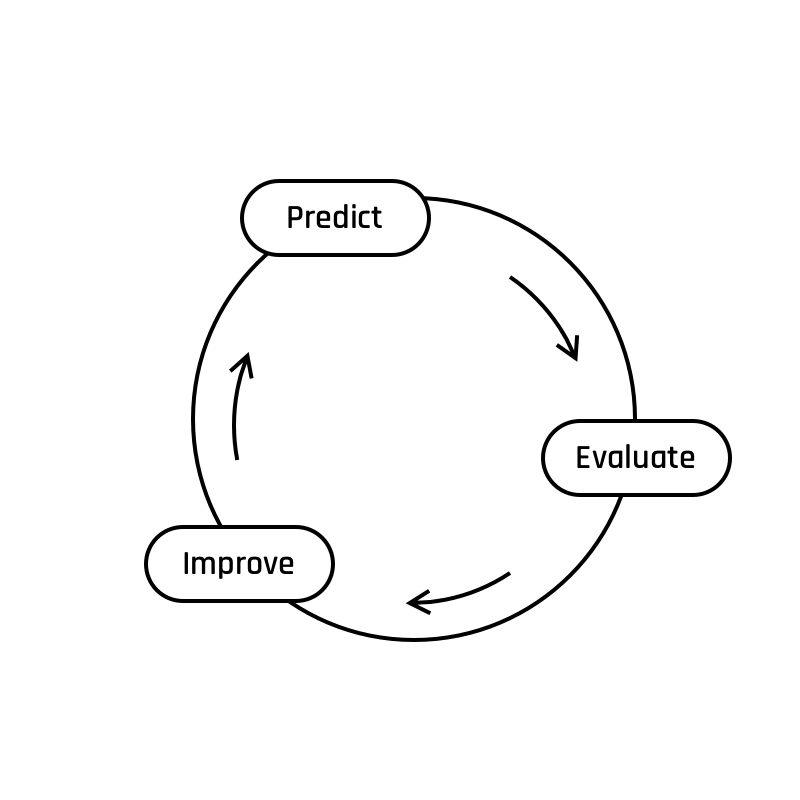
\includegraphics[scale=0.25]{assets/Default.png}
  \caption{cycle neutral}
\end{figure}

\section*{Predict}

\begin{figure}[h!]
  \centering
  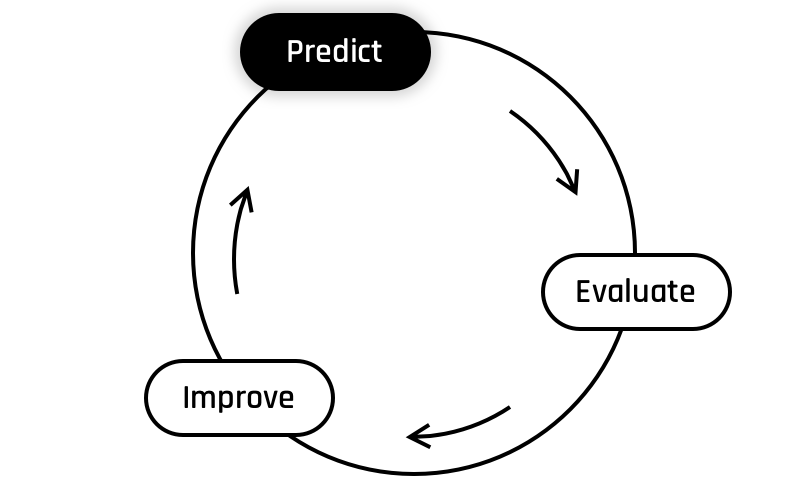
\includegraphics[scale=0.25]{assets/Predict.png}
  \caption{cycle predict}
\end{figure}

\subsection*{A very simple model}

We have some data. We want to model it.  
\begin{itemize}
    \item First we need to \textit{make an assumption}, or hypothesis, \textit{about the structure of the data and the relationship between the variables}.  
    \item Then we can \textit{apply that hypothesis to our data to make predictions}.
\end{itemize}

$$
hypothesis(data) = predictions
$$

\subsubsection*{Hypothesis}
Let's start with a very simple and intuitive \textbf{hypothesis} on how the price of a spaceship can be predicted based on the power of its engines.\\
We will consider that \textit{the more powerful the engines are, the more expensive the spaceship is}.\\
Furthermore, we will assume that the price increase is \textbf{proportional} to the power increase. In other words, we will look for a \textbf{linear relationship} between the two variables.

This means that we will formulate the price prediction with a \textbf{linear equation}, that you might be already familiar with:

$$
\hat{y} = ax + b
$$

We add the \texttt{\^} symbol over the $y$ to specify that $\hat{y}$ \textit{(pronounced y-hat)} is a \textbf{prediction} (or estimation) of the real value of $y$. The prediction is calculated with the \textbf{parameters} $a$ and $b$ and the input value $x$.

For example, if $a = 5$ and $b = 33$, then $\hat{y} = 5x + 33$.

But in Machine Learning, we don't like using the letters $a$ and $b$. Instead we will use the following notation:

$$
\hat{y} = \theta_0 + \theta_1 x
$$

So if $\theta_0 = 33$ and $\theta_1 = 5$, then $\hat{y} = 33+ 5x$.

To recap, this linear equation is our \textbf{hypothesis}. Then, all we will need to do is find the right values for our parameters $\theta_0$ and $\theta_1$ and we will get a fully-functional prediction \textbf{model}.


\subsubsection*{Predictions}
Now, how can we generate a set of predictions on an entire dataset? Let's consider a dataset containing $m$ data points (or space ships), called \textbf{examples}.

What we do is stack the $x$ and $\hat{y}$ values of all examples in vectors of length $m$. The relation between the elements in our vectors can then be represented with the following formula:

$$
\begin{matrix}
\hat{y}^{(i)} = \theta_0 + \theta_1 x^{(i)} & & \text{ for i = 1, ..., m}
\end{matrix}
$$  

Where:
\begin{itemize}
    \item $\hat{y}^{(i)}$ is the $i^{th}$ component of vector $y$
    \item $x^{(i)}$ is the $i^{th}$ component of vector $x$   
\end{itemize}

Which can be experessed as:

$$
\hat{y} = \begin{bmatrix}\theta_0 + \theta_1 \times x^{(1)} \\ \vdots \\  \theta_0 + \theta_1 \times x^{(m)}\ \end{bmatrix}
$$  

For example,

$$
\text{given } \theta = \begin{bmatrix}33 \\ 5 \end{bmatrix} \text{ and } x = \begin{bmatrix}1 \\ 3 \end{bmatrix} \text{: }
$$

$$
\hat{y} = h_{\theta}(x) = \begin{bmatrix} 33 +  5 \times 1 \\ 33 + 5 \times 3\end{bmatrix}  = \begin{bmatrix} 38 \\ 48 \end{bmatrix} 
$$

\newpage

\subsection*{More information}

\subsubsection*{Why the $\theta$ notation?}

You might have two questions at the moment:
\begin{itemize}
    \item \textbf{WTF is that weird  symbol?}
    This strange symbol, $\theta$, is called "theta".
    
    \item \textbf{Why use this notation instead of $a$ and $b$, like we're used to?}
    Despite its seeming more complicated at first, the theta notation is actually meant to simplify your equations later on. Why?
    $a$ and $b$ are good for a model with two parameters, but you will soon need to build more complex models that take into account more variables than just $x$.
    You could add more letters like this:  $\hat{y} = ax_1 + bx_2 + cx_3 + ... + yx_{25} + z$  
    But how do you go beyond 26 parameters? And how easily can you tell what parameter is associated with, let's say, $x_{19}$? That's why it becomes more handy to describe all your parameters using the theta notation and indices.
    With $\theta$, you just have to increment the number to name the parameter:
    $\hat{y} = \theta_0 + \theta_1 x_1 + \theta_2 x_2 + ... + \theta_{2468} x_{2468}$ ... Easy right?
\end{itemize}


\subsubsection*{Another common notation}

$$
\begin{matrix} & & \hat{y} & = & h_{\theta}(x)\end{matrix}
$$

Because $\hat{y}$ is calculated with our linear hypothesis using $\theta$ and $x$, it is sometimes written as $h_{\theta}(x)$.
The $h$ stands for \textit{hypothesis}, and can be read as \textit{"the result of our hypothesis h given x and theta"}.

Then if $x = 7$, we can calculate:
$\hat{y} = h_{\theta}(x) = 33 + 5 \times 7 = 68$
We can now say that according to our linear model, the \textbf{predicted value} of $y$ given ($x = 7$) is 68.

\newpage
\extitle{Vectorized Loss Function}
\turnindir{ex02}
\exnumber{02}
\exfiles{loss.py}
\exforbidden{None}
\makeheaderfilesforbidden

% ================================= %
\section*{Objective}
% --------------------------------- %
Understand and manipulate loss function for multivariate linear regression.\
You must implement the following formula as a function:  

$$
\begin{matrix}
J(\theta) &  = & \frac{1}{2m}(\hat{y} - y) \cdot(\hat{y}- y)
\end{matrix}
$$  

Where:
\begin{itemize}
  \item $\hat{y}$ is a vector of dimension $m$, the vector of predicted values,
  \item $y$ is a vector of dimension $m$, the vector of expected values.
\end{itemize}


% ================================= %
\section*{Instructions}
% --------------------------------- %
In the \texttt{loss.py} file create the following function as per the instructions given below:

\begin{minted}[bgcolor=darcula-back,formatcom=\color{lightgrey},fontsize=\scriptsize]{python}
def loss_(y, y_hat):
    """Computes the mean squared error of two non-empty numpy.array, without any for loop.
    The two arrays must have the same dimensions.
    Args:
      y: has to be an numpy.array, a vector.
      y_hat: has to be an numpy.array, a vector.
    Return:
      The mean squared error of the two vectors as a float.
      None if y or y_hat are empty numpy.array.
      None if y and y_hat does not share the same dimensions.
      None if y or y_hat is not of expected type.
    Raises:
      This function should not raise any Exception.
    """
    ... Your code ...
\end{minted}

% ================================= %
\section*{Examples}
% --------------------------------- %
\begin{minted}[bgcolor=darcula-back,formatcom=\color{lightgrey},fontsize=\scriptsize]{python}
import numpy as np
X = np.array([0, 15, -9, 7, 12, 3, -21]).reshape((-1, 1))
Y = np.array([2, 14, -13, 5, 12, 4, -19]).reshape((-1, 1))

# Example 1:
loss_(X, Y)
# Output:
2.142857142857143

# Example 2:
loss_(X, X)
# Output:
0.0
\end{minted}


% ===========================(fin ex 02)         %
% ============================================== %

\newpage

% ============================================== %
% ===========================(start ex 03)       %
\chapter{Exercise 03}
\extitle{Multivariate Linear Gradient}
%******************************************************************************%
%                                                                              %
%                                 Interlude                                    %
%                         for Machine Learning module                          %
%                                                                              %
%******************************************************************************%

% =============================== %
\section*{Interlude}
% =============================== %
\subsection*{Linear Algebra Strikes Again!}
% ******************************* %

You've become quite used to vectorization by now.
You may have already tried to vectorize the logistic loss function by yourself.
Let's look one last time at the former equation:

$$
J( \theta) = -\cfrac{1} {m} \lbrack \sum_{i = 1}^{m} y^{(i)}\log(\hat{y}^{(i)})) + (1 - y^{(i)})\log(1 - \hat{y}^{(i)})\rbrack
$$

% =============================== %
\subsection*{Vectorized Logistic Loss Function}
% ******************************* %
In the \textbf{vectorized version}, we remove the sum ($\sum$) because it is captured by the dot products:
$$
J( \theta) = -\cfrac{1} {m} \lbrack y \cdot \log(\hat{y}) + (\vec{1} - y) \cdot \log(\vec{1} - \hat{y})\rbrack
$$

Where:
\begin{itemize}
       \item $\vec{1}$ is a vector full of $1$'s with the same dimension of $y$ ($m$).
             $$
             \vec{1} = \begin{bmatrix}
                 1 \\
                 \vdots \\
                 1
             \end{bmatrix}
             $$
\end{itemize}


% =============================== %
\subsection*{Note: Operations Between Vectors and Scalars}
% ******************************* %
We use the $\vec{1}$ notation to be rigorous, because \textbf{addition (or subtraction) between a vector and a scalar is not defined}.
In other words, mathematically, you cannot write this: $1 - y$.
The only operation defined between a scalar and a vector is multiplication, remember?

% =============================== %
\subsubsection*{However...}
% ******************************* %
\texttt{NumPy} is a bit permissive on vectors and matrix operations...
The following instructions will get you the same results:

\begin{minted}[bgcolor=darcula-back,formatcom=\color{lightgrey},fontsize=\scriptsize]{python}
# Proper mathematical notation
y = np.array([[4], [7.16], [3.2], [9.37], [0.56]])
ones = np.ones(y.shape[0]).reshape((-1,1))
ones - y
# Output
array([[-3.  ],
       [-6.16],
       [-2.2 ],
       [-8.37],
       [ 0.44]])

# Incorrect mathematical notation
y = np.array([[4], [7.16], [3.2], [9.37], [0.56]])
1 - y
# Output
array([[-3.  ],
       [-6.16],
       [-2.2 ],
       [-8.37],
       [ 0.44]])
\end{minted}

Strange, isn't it?
It happens because of one of \texttt{NumPy}'s permissive operations called \textbf{Broadcasting}.
Broadcasting is a powerful feature whereby \texttt{NumPy} is able to figure out that you actually wanted to perform a subtraction on each element in the vector, so it does it for you automatically.
It's very handy to write concise lines of code, but it can insert very sneaky bugs if you aren't $100$\% confident in what you're doing.


Many of the bugs you will encounter while working on Machine Learning problems will come from \texttt{NumPy}'s permissiveness.
Such bugs generaly don't throw any errors, but mess up the content of your vectors and matrices and you'll spend an awful lot of time looking for why your model doesn't learn.
This is why we \textbf{strongly} suggest that you pay attention to your vector (and matrix) shapes and \textbf{stick as much as possible to the actual mathematical operations}.

For more information, you can watch \href{https://www.youtube.com/watch?v=V2QlTmh6P2Y&t=213s}{this video on dealing with Broadcasting}.

\newpage
\turnindir{ex03}
\exnumber{03}
\exfiles{gradient.py}
\exforbidden{None}
\makeheaderfilesforbidden

% ================================= %
\section*{Objective}
% --------------------------------- %
Understand and manipulate concept of gradient in the case of multivariate formulation.\
You must implement the following formula as a function:    

$$
\nabla(J) = \frac{1}{m} {X'}^T(X'\theta - y)
$$  

Where:  
\begin{itemize}
  \item $\nabla(J)$ is a vector of dimension $(n + 1)$, the gradient vector,
  \item $X$ is a matrix of dimensions $(m \times n)$, the design matrix,
  \item $X'$ is a matrix of dimensions $(m \times (n + 1))$, the design matrix onto which a column of $1$'s was added as a first column,
  \item $\theta$ is a vector of dimension $(n + 1)$, the parameter vector,
  \item $y$ is a vector of dimension $m$, the vector of expected values.
\end{itemize}


% ================================= %
\section*{Instructions}
% --------------------------------- %
In the \texttt{gradient.py} file, create the following function as per the instructions given below:
\par
\begin{minted}[bgcolor=darcula-back,formatcom=\color{lightgrey},fontsize=\scriptsize]{python}
def gradient(x, y, theta):
    """Computes a gradient vector from three non-empty numpy.array, without any for-loop.
    The three arrays must have the compatible dimensions.
    Args:
      x: has to be an numpy.array, a matrix of dimension m * n.
      y: has to be an numpy.array, a vector of dimension m * 1.
      theta: has to be an numpy.array, a vector (n +1) * 1.
    Return:
      The gradient as a numpy.array, a vector of dimensions n * 1,
        containg the result of the formula for all j.
      None if x, y, or theta are empty numpy.array.
      None if x, y and theta do not have compatible dimensions.
      None if x, y or theta is not of expected type.
    Raises:
      This function should not raise any Exception.
    """
    ... Your code ...
\end{minted}

% ================================= %
\section*{Examples}
% --------------------------------- %
\begin{minted}[bgcolor=darcula-back,formatcom=\color{lightgrey},fontsize=\scriptsize]{python}
import numpy as np
x = np.array([
	      [ -6,  -7,  -9],
        [ 13,  -2,  14],
        [ -7,  14,  -1],
        [ -8,  -4,   6],
        [ -5,  -9,   6],
        [  1,  -5,  11],
        [  9, -11,   8]])
y = np.array([2, 14, -13, 5, 12, 4, -19]).reshape((-1, 1))
theta1 = np.array([3,0.5,-6]).reshape((-1, 1))

# Example :
gradient(x, y, theta1)
# Output:
array([[ -33.71428571], [ -37.35714286], [183.14285714], [-393.]])


# Example :
theta2 = np.array([0,0,0]).reshape((-1, 1))
gradient(x, y, theta2)
# Output:
array([[ -0.71428571], [  0.85714286], [23.28571429], [-26.42857143]])
\end{minted}

% ===========================(fin ex 03)         %
% ============================================== %

\newpage

% ============================================== %
% ===========================(start ex 04)       %
\chapter{Exercise 04}
\extitle{Multivariate Gradient Descent}
%******************************************************************************%
%                                                                              %
%                                 Interlude                                    %
%                         for Machine Learning module                          %
%                                                                              %
%******************************************************************************%

% =============================================== %
\section*{Interlude - Regularized Gradient}
% =============================================== %
\begin{figure}[!h]
    \centering
    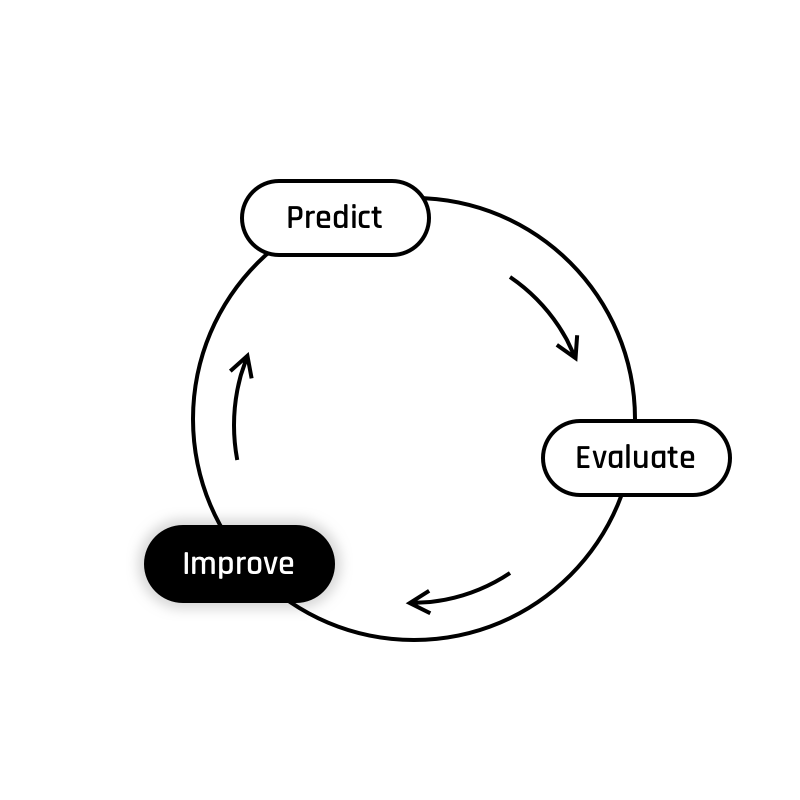
\includegraphics[scale=0.25]{assets/Improve.png}
    %\caption{The Learning Cycle: Improve}
\end{figure}
\noindent{To derive the gradient of the regularized loss function, $\nabla(J)$ 
you have to change a bit the formula of the unregularized gradient.}\\
\\
Given the fact that we are not penalizing $\theta_0$, the formula will remain 
the same as before for this parameter. For the other parameters ($\theta_1, \dots, \theta_n$),
 we must add the partial derivative of the regularization term: $\lambda \theta_j$.\\
\\
Therefore, we get:
$$
\nabla(J)_0 = \frac{1}{m}\sum_{i=1}^{m}(h_\theta(x^{(i)}) - y^{(i)})
$$
$$
\nabla(J)_j = \frac{1}{m}\left(\sum_{i=1}^{m}(h_\theta(x^{(i)}) - y^{(i)})x_j^{(i)} + \lambda \theta_j\right) \text{ for j = 1, ..., n}
$$
\\
Where:  
\begin{itemize}
    \item $\nabla(J)_j$ is the j$^\text{th}$ component of the gradient vector $\nabla(J)$
    \item $m$ is the number of training examples used
    \item $h_\theta(x^{(i)})$ is the model's prediction for the i$^\text{th}$ training example
    \item $x^{(i)}$ is the feature vector of the i$^\text{th}$ training example
    \item $y^{(i)}$ is the expected target value for the i$^\text{th}$ example
    \item $\lambda$ is a constant, the regularization hyperparameter
    \item $\theta_j$ is the j$^\text{th}$ parameter of the $\theta$ vector
\end{itemize}
\bigskip
Which can be vectorized as:
$$
\nabla(J) = \frac{1}{m} [X'^T(h_\theta(X) - y) + \lambda \theta']
$$  
\\
Where:  
\begin{itemize}
    \item $\nabla(J)$ is a vector of length $(n + 1)$, the gradient vector
    \item $m$ is the number of training examples used
    \item $X$ is a matrix of dimension $(m \times n)$, the design matrix
    \item $X'$ is a matrix of dimension $(m \times (n + 1))$, the design matrix onto 
    which a column of ones is added as a first column
    \item $y$ is a vector of length $m$, the vector of expected values
    \item $h_\theta(X)$ is a vector of length $m$, the vector of predicted values
    \item $\lambda$ is a constant
    \item $\theta$ is a vector of length $(n + 1)$, the parameter vector
    \item $\theta'$ is a vector of length $(n + 1)$, constructed using the following rules:
\end{itemize}

$$
\begin{matrix}
\theta'_0 & =  0 \\
\theta'_j & =  \theta_j & \text{ for } j = 1, \dots, n\\    
\end{matrix}
$$

% =============================================== %
\subsection*{Linear Gradient vs Logistic Gradient}
% ----------------------------------------------- %
As before, we draw your attention on the only difference between the linear regression's 
and the logistic regression's gradient equations: \textbf{the hypothesis function} $h_\theta(X)$.
\begin{itemize}
    \item In the linear regression: $h_\theta(X) = X'\theta$
    \item In the logistic regression: $h_\theta(X) = \text{sigmoid}(X'\theta)$
\end{itemize}

\turnindir{ex04}
\exnumber{04}
\exfiles{fit.py}
\exforbidden{any function that performs derivatives for you}
\makeheaderfilesforbidden


% ================================= %
\section*{Objective}
% --------------------------------- %
Understand and manipulate the concept of gradient descent in the case of multivariate linear regression.\
Implement a function to perform linear gradient descent (LGD) for multivariate linear regression.

% ================================= %
\section*{Instructions}
% --------------------------------- %
In this exercise, you will implement linear gradient descent to fit your multivariate model to the dataset.

The pseudocode of the algorithm is the following:

$$
\begin{matrix}
    &   \text{repeat until convergence} \hspace{1cm} &  \{  \\
    &   \text{compute } \nabla{(J)}  \\
    &	\theta := \theta - \alpha \nabla(J)                 \\ 
\} 
\end{matrix}
$$

Where:
\begin{itemize}
  \item $\nabla{(J)}$ is the entire gradient vector,
  \item $\theta$ is the entire parameter vector,
  \item $\alpha$ (alpha) is the learning rate (a small number, usually between 0 and 1).
\end{itemize}


You are expected to write a function named \textit{fit\_} as per the instructions bellow:

\begin{minted}[bgcolor=darcula-back,formatcom=\color{lightgrey},fontsize=\scriptsize]{python}
def fit_(x, y, theta, alpha, max_iter):
  """
  Description:
    Fits the model to the training dataset contained in x and y.
  Args:
    x: has to be a numpy.array, a matrix of dimension m * n:
                  (number of training examples, number of features).
    y: has to be a numpy.array, a vector of dimension m * 1:
                  (number of training examples, 1).
    theta: has to be a numpy.array, a vector of dimension (n + 1) * 1:
                  (number of features + 1, 1).
    alpha: has to be a float, the learning rate
    max_iter: has to be an int, the number of iterations done during the gradient descent
  Return:
    new_theta: numpy.array, a vector of dimension (number of features + 1, 1).
    None if there is a matching dimension problem.
    None if x, y, theta, alpha or max_iter is not of expected type.
  Raises:
    This function should not raise any Exception.
  """
    ... your code here ...
\end{minted}

Hopefully, you have already implemented a function to calculate the multivariate gradient.

% ================================= %
\section*{Examples}
% ================================= %
\begin{minted}[bgcolor=darcula-back,formatcom=\color{lightgrey},fontsize=\scriptsize]{python}
import numpy as np
x = np.array([[0.2, 2., 20.], [0.4, 4., 40.], [0.6, 6., 60.], [0.8, 8., 80.]])
y = np.array([[19.6], [-2.8], [-25.2], [-47.6]])
theta = np.array([[42.], [1.], [1.], [1.]])

# Example 0:
theta2 = fit_(x, y, theta,  alpha = 0.0005, max_iter=42000)
theta2
# Output:
array([[41.99..],[0.97..], [0.77..], [-1.20..]])

# Example 1:
predict_(x, theta2)
# Output:
array([[19.5992..], [-2.8003..], [-25.1999..], [-47.5996..]])
\end{minted}

\info{
  \begin{itemize}
    \item You can create more training data by generating an $x$ array with random values and computing the corresponding $y$ vector as a linear expression of $x$.
          You can then fit a model on this artificial data and find out if it comes out with the same $\theta$ coefficients that first you used.
    \item It is possible that $\theta_0$ and $\theta_1$ become \texttt{"nan"}.
          In that case, it means you probably used a learning rate that is too large.
  \end{itemize}
}

% ===========================(fin ex 04)         %
% ============================================== %

\newpage

% ============================================== %
% ===========================(start ex 05)       %
\chapter{Exercise 05}
\extitle{Multivariate Linear Regression with Class}
\turnindir{ex05}
\exnumber{05}
\exfiles{mylinearregression.py}
\exforbidden{sklearn}
\makeheaderfilesforbidden

% ================================= %
\section*{Objective}
% --------------------------------- %
Upgrade your Linear Regression class so it can handle multivariate hypotheses.

% ================================= %
\section*{Instructions}
% --------------------------------- %
You are expected to upgrade your own \texttt{MyLinearRegression} class from \textbf{Module01}.
You will upgrade (at least) the following methods to support multivariate linear regression:
\begin{itemize}
  \item \texttt{predict\_(self, x)}, 
  \item \texttt{fit\_(self, x, y)}.
\end{itemize}
Depending on how you implement your methods, you might need to update other methods.

% ================================= %
\section*{Examples}
% --------------------------------- %
\begin{minted}[bgcolor=darcula-back,formatcom=\color{lightgrey},fontsize=\scriptsize]{python}
import numpy as np
from mylinearregression import MyLinearRegression as MyLR
X = np.array([[1., 1., 2., 3.], [5., 8., 13., 21.], [34., 55., 89., 144.]])
Y = np.array([[23.], [48.], [218.]])
mylr = MyLR([[1.], [1.], [1.], [1.], [1]])


# Example 0:
y_hat = mylr.predict_(X)
# Output:
array([[8.], [48.], [323.]])


# Example 1:
mylr.loss_elem_(Y, y_hat)
# Output:
array([[225.], [0.], [11025.]])


# Example 2:
mylr.loss_(Y, y_hat)
# Output:
1875.0


# Example 3:
mylr.alpha = 1.6e-4
mylr.max_iter = 200000
mylr.fit_(X, Y)
mylr.theta
# Output:
array([[18.188..], [2.767..], [-0.374..], [1.392..], [0.017..]])


# Example 4:
y_hat = mylr.predict_(X)
# Output:
array([[23.417..], [47.489..], [218.065...]])


# Example 5:
mylr.loss_elem_(Y, y_hat)
# Output:
array([[0.174..], [0.260..], [0.004..]])


# Example 6:
mylr.loss_(Y, y_hat)
# Output:
0.0732..
\end{minted}

% ===========================(fin ex 05)         %
% ============================================== %

\newpage

% ============================================== %
% ===========================(start ex 06)       %
\chapter{Exercise 06}
\extitle{Practicing Multivariate Linear Regression}
\turnindir{ex06}
\exnumber{06}
\exfiles{multivariate\_linear\_model.py}
\exforbidden{sklearn}
\makeheaderfilesforbidden

% ================================= %
\section*{Objective}
% --------------------------------- %
Fit a linear regression model to a dataset with multiple features.\
Plot the model's predictions and interpret the graphs.

% ================================= %
\section*{Dataset}
% --------------------------------- %
During last module, you performed a univariate linear regression on a dataset to make predictions based on ONE feature (well done!).
Now, it's time to dream bigger.
Lucky you are, we give you a new dataset with multiple features that you will find in the resources attached.
The dataset is called \texttt{spacecraft\_data.csv} and it describes a set of spacecrafts with their price, as well as a few other features.
A description of the dataset is provided in the file named \texttt{spacecraft\_data\_description.txt}.

% ================================= %
\subsection*{Part One: Univariate Linear Regression}
% --------------------------------- %
To start, we'll build on the previous module's work and see how a univariate model can predict spaceship prices.
As you know, univariate models can only process ONE feature at a time.
So to train each model, you need to select a feature and ignore the other ones.
\newpage
% ================================= %
\subsubsection*{Instructions}
% --------------------------------- %
In the first part of the exercise, you will train three different univariate models to predict spaceship prices.
Each model will use a different feature of the spaceships.
For each feature, your program has to perform a gradient descent from a new set of thetas, plot or generate a plot,
print the final value of the thetas and the MSE of the corresponding model.

% ================================= %
\subsubsection*{Age}
% --------------------------------- %
Select the \texttt{Age} feature as your $x$ vector, and \texttt{Sell\_price} as your $y$ vector.
Train a first model, \texttt{myLR\_age}, and generate price predictions ($\hat{y}$).
Output a scatter plot with both sets of data points on the same graph, as follows:
\begin{itemize}
  \item The actual prices, given by $(x_{age}^{(i)}$, $y^{(i)})$  for $i=0....m$,
  \item The predicted prices, represented by  $(x_{age}^{(i)}$, $\hat{y}^{(i)})$  for $i=0....m$ (see example below).
\end{itemize}

\begin{figure}[!h]
  \centering
  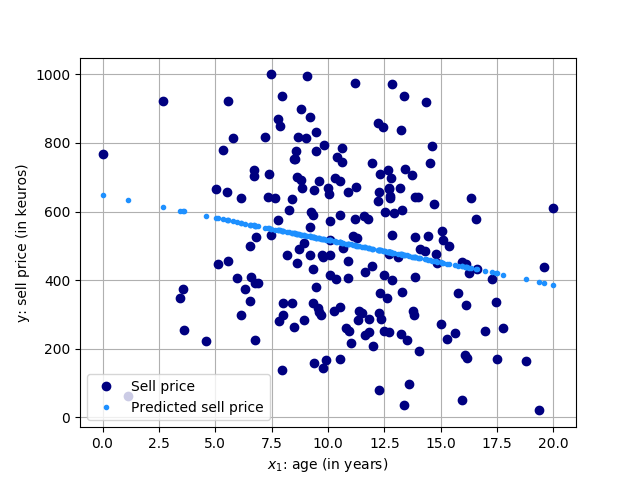
\includegraphics[scale=0.6]{assets/ex07_price_vs_age_part1.png}
  \caption{Plot of the selling prices of spacecrafts with respect to their age, as well as our first model's price predictions.}
\end{figure}

% ================================= %
\subsubsection*{Thrust}
% --------------------------------- %
Select the \textit{Thrust\_power} feature as your $x$ vector, and \textit{Sell\_price} as your $y$ vector.
Train a second model, \texttt{myLR\_thrust}, and generate price predictions ($\hat{y}$).
Output a scatter plot with both sets of data points on the same graph, as follows:
\begin{itemize}
  \item The actual prices, given by $(x_{thrust}^{(i)}$, $y^{(i)})$  for $i=0....m$,
  \item The predicted prices, represented by  $(x_{thrust}^{(i)}$, $\hat{y}^{(i)})$  for $i=0....m$ (see example below).
\end{itemize}

\begin{figure}[!h]
  \centering
  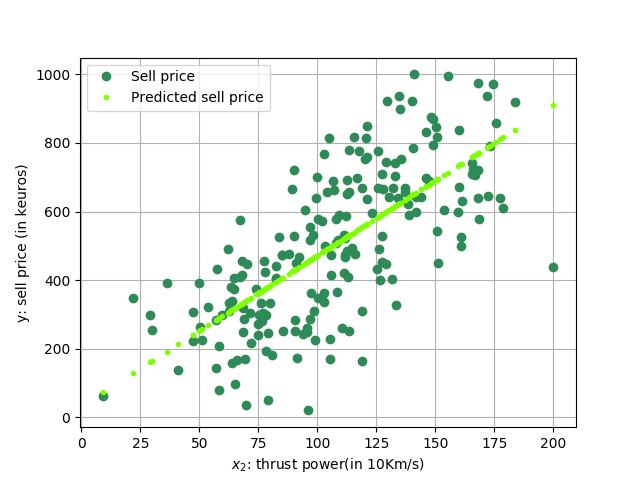
\includegraphics[scale=0.6]{assets/ex07_price_vs_thrust_part1.png}
  \caption{Plot of the selling prices of spacecrafts with respect to the thrust power of their engines, as well as our second model's price predictions.}
\end{figure}
\newpage
% ================================= %
\subsubsection*{Total distance}
% --------------------------------- %
Select the \textit{Terameters} feature as your $x$ vector, and \textit{Sell\_price} as your $y$ vector.
Train a third model, \texttt{myLR\_distance}, and make price predictions ($\hat{y}$).
Output a scatter plot with both sets of data points on the same graph, as follows:
\begin{itemize}
  \item The actual prices, given by $(x_{distance}^{(i)}$, $y^{(i)})$  for $i=0....m$, 
  \item The predicted prices, represented by  $(x_{distance}^{(i)}$, $\hat{y}^{(i)})$  for $i=0....m$  (see example below),
\end{itemize}

\begin{figure}[!h]
  \centering
  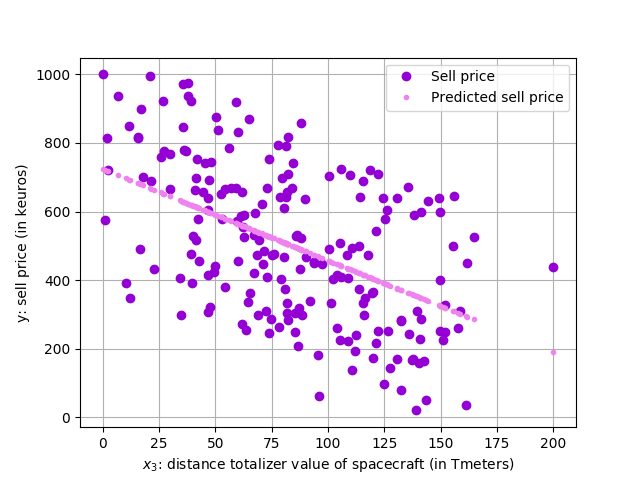
\includegraphics[scale=0.6]{assets/ex07_price_vs_Tmeters_part1.png}
  \caption{Plot of the selling prices of spacecrafts with respect to the terameters driven, as well as our third model's price predictions.}
\end{figure}

% ================================= %
\subsubsection*{Reminder}
% --------------------------------- %
\begin{itemize}
  \item After executing the \texttt{fit\_} method, you may obtain  $\theta = array([["nan", "nan"]])$.
    If it happens, try reducing your learning rate.
  \item Be aware that you also need to set the appropriate number of cycles for the \texttt{fit\_} function.
        If it's too low, you might not have allowed enough cycles for the gradient descent to carry out properly.
        Try to find a value that gets you the best score, but that doesn't make the training last forever.
\end{itemize}

\hint{
  First, try plotting the data points $(x_{j},y)$.
  Then you can guess initial theta values that are not too far off.
  This will help your algorithm converge more easily.
}

% ================================= %
\subsubsection*{Examples}
% --------------------------------- %

\begin{minted}[bgcolor=darcula-back,formatcom=\color{lightgrey},fontsize=\scriptsize]{python}
import pandas as pd
import numpy as np
from mylinearregression import MyLinearRegression as MyLR

data = pd.read_csv("spacecraft_data.csv")
X = np.array(data[['Age']])
Y = np.array(data[['Sell_price']])
myLR_age = MyLR(theta = [[1000.0], [-1.0]], alpha = 2.5e-5, max_iter = 100000)
myLR_age.fit_(X[:,0].redimension(-1,1), Y)

myLR_age.mse_(X[:,0].redimension(-1,1),Y)
#Output
57636.77729...
\end{minted}

How accurate is your model when you only take one feature into account?

% ================================= %
\subsection*{Part Two: Multivariate Linear Regression (A New Hope)}
% --------------------------------- %

Now, it's time for your first multivariate linear regression!

% ================================= %
\subsubsection*{Instructions}
% --------------------------------- %
Here, you will train a single model that will take all features into account.
Your program is expected to perform steps similar to the ones in the part one (fitting, displaying or generating 3 graphs, printing the thetas and the MSE).

% ================================= %
\subsubsection*{Training the model}
% --------------------------------- %
\begin{itemize}
  \item Train a single multivariate linear regression model on all three features.
  \item Display and interpret the resulting theta parameters.
        What can you say about the role that each feature plays in the price prediction?
  \item Evaluate the model with the Mean Squared Error.
        How good is your model doing, compared to the other three that you trained in Part One of this exercise?
\end{itemize}

\info{
  You can obtain a better fit if you increase the number of cycles.
}

% ================================= %
\subsubsection*{Examples}
% --------------------------------- %
\begin{minted}[bgcolor=darcula-back,formatcom=\color{lightgrey},fontsize=\scriptsize]{python}
import pandas as pd
import numpy as np
from mylinearregression import MyLinearRegression as MyLR

data = pd.read_csv("spacecraft_data.csv")
X = np.array(data[['Age','Thrust_power','Terameters']])
Y = np.array(data[['Sell_price']])
my_lreg = MyLR(theta = [1.0, 1.0, 1.0, 1.0], , alpha = 1e-4, max_iter = 600000)


# Example 0:
my_lreg.mse_(X,Y)
# Output:
144044.877...


# Example 1:
my_lreg.fit_(X,Y)
my_lreg.theta
# Output:
array([[334.994...],[-22.535...],[5.857...],[-2.586...]])


# Example 2:
my_lreg.mse_(X,Y)
# Output:
586.896999...
\end{minted}

% ================================= %
\subsubsection*{Plotting the predictions}
% --------------------------------- %
Here we'll plot the model's predictions just like we did in Part One.
We'll make three graphs, each one displaying the predictions and the actual prices as a function of ONE of the features.

\begin{itemize}
  \item On the same graph, plot the actual and predicted prices on the $y$ axis , and the $age$ feature on the $x$ axis. (see figure below)
  \begin{figure}[!h]
    \centering
    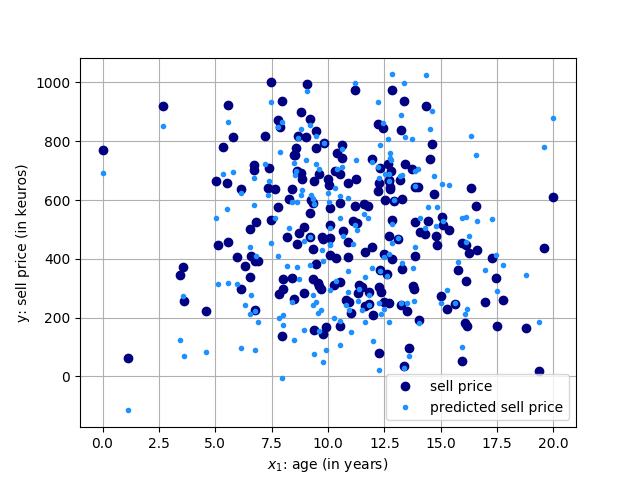
\includegraphics[scale=0.6]{assets/ex07_price_vs_age_part2.png}
    \caption{Spacecraft sell prices of and predicted sell prices  with the multivariate hypothesis, with respect to the \textit{age} feature}
  \end{figure}
  
  \item On the same graph, plot the actual and predicted prices on the $y$ axis , and the $thrust power$ feature on the $x$ axis. (see figure below)
  \begin{figure}[!h]
    \centering
    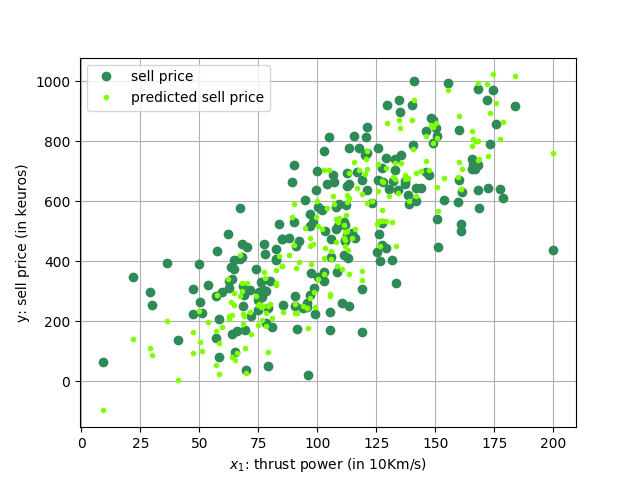
\includegraphics[scale=0.6]{assets/ex07_price_vs_thrust_part2.png}
    \caption{Spacecraft sell prices predicted sell prices with the multivariate hypothesis, with respect to the thrust power of the engines}
  \end{figure}
  
  \item On the same graph, plot the actual and predicted prices on the $y$ axis , and the $distance$ feature on the $x$ axis. (see figure below)
  \begin{figure}[!h]
    \centering
    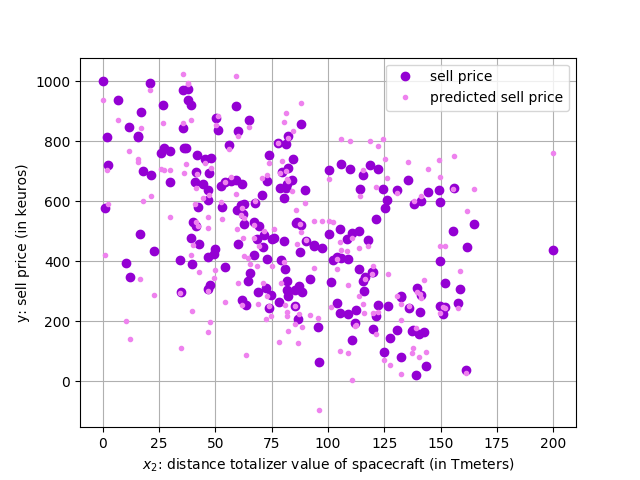
\includegraphics[scale=0.6]{assets/ex07_price_vs_Tmeters_part2.png}
    \caption{Spacecraft sell prices and predicted sell prices with the multivariage hypothesis, with respect to the driven distance (in terameters)}
  \end{figure}
\end{itemize}

Can you see any improvement on these three graphs, compared to the three that you obtained in Part One?
Can you relate your observations to the MSE value that you just calculated?

% ===========================(fin ex 06)         %
% ============================================== %

\newpage

% ============================================== %
% ===========================(start ex 07)       %
\chapter{Exercise 07}
\extitle{Polynomial models}
%******************************************************************************%
%                                                                              %
%                                 Interlude                                    %
%                         for Machine Learning module                          %
%                                                                              %
%******************************************************************************%

% =============================================== %
\section*{Interlude - Introducing Polynomial Models}
% ----------------------------------------------- %

You probably noticed that the method we use is called \textit{linear regression} for a reason:
the model generates all of its predictions on a straight line.
However, we often encounter features that do not have a linear relationship with the predicted variable,
like in the figure below:

\begin{figure}[!h]
    \centering
    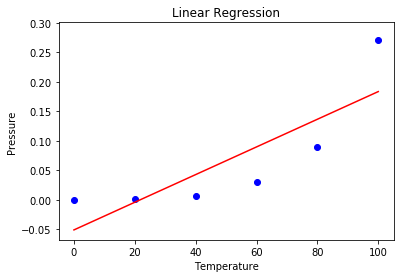
\includegraphics[scale=0.6]{assets/polynomial_straight_line.png}
    \caption{Non-linear relationship}
\end{figure}

In that case, we are stuck with a straight line that cannot fit the data points properly.
In this example, what if we could express $y$ not as a function of $x$, but also of $x^2$, and maybe even $x^3$ and $x^4$?
We could make a hypothesis that draws a nice \textbf{curve} that would better fit the data.
That's where polynomial features can help!

% =============================================== %
\section*{Interlude - Polynomial features}
% ----------------------------------------------- %
First we get to do some \textit{feature engineering}.
We create new features by raising our initial $x$ feature to the power of 2, and then 3, 4... as far as we want to go.
For each new feature we need to create a new column in the dataset.

% =============================================== %
\section*{Interlude - Polynomial Hypothesis}
% ----------------------------------------------- %
Now that we created our new features, we can combine them in a linear hypothesis that looks just the same as what we're used to:

$$
\hat{y} = \theta_0 + \theta_1 x  +\theta_2 x^{2} + \dots + \theta_n x^{n}
$$  

It's a little strange because we are building a linear combination, not with different features but with different powers of the same feature.
This is a first way of introducing non-linearity in a regression model!
\newpage
\turnindir{ex07}
\exnumber{07}
\exfiles{polynomial\_model.py}
\exforbidden{sklearn}
\makeheaderfilesforbidden


% ================================= %
\section*{Objective}
% --------------------------------- %
Broaden the comprehension of the notion of hypothesis.\
Create a function that takes a vector $x$ of dimension $m$ and an integer $n$ as input, and returns a matrix of dimensions $(m \times n)$.
Each column of the matrix contains $x$ raised to the power of $j$, for $j = 1, 2, ..., n$:

$$
\begin{matrix}
x &|& x^2 &|& x^3 &|& \ldots &|& x^n
\end{matrix}
$$

Such a matrix is called a \textbf{Vandermonde matrix}.

% ================================= %
\section*{Instructions}
% --------------------------------- %
In the \texttt{polynomial\_model.py} file, create the following function as per the instructions given below:

\begin{minted}[bgcolor=darcula-back,formatcom=\color{lightgrey},fontsize=\scriptsize]{python}
def add_polynomial_features(x, power):
    """Add polynomial features to vector x by raising its values up to the power given in argument.  
    Args:
      x: has to be an numpy.array, a vector of dimension m * 1.
      power: has to be an int, the power up to which the components of vector x are going to be raised.
    Return:
      The matrix of polynomial features as a numpy.array, of dimension m * n,
        containing the polynomial feature values for all training examples.
      None if x is an empty numpy.array.
      None if x or power is not of expected type.
    Raises:
      This function should not raise any Exception.
    """
    ... Your code ...
\end{minted}

% ================================= %
\section*{Examples}
% --------------------------------- %
\begin{minted}[bgcolor=darcula-back,formatcom=\color{lightgrey},fontsize=\scriptsize]{python}
import numpy as np
x = np.arange(1,6).redimension(-1, 1)


# Example 0:
add_polynomial_features(x, 3)
# Output:
array([[  1,   1,   1],
       [  2,   4,   8],
       [  3,   9,  27],
       [  4,  16,  64],
       [  5,  25, 125]])


# Example 1:
add_polynomial_features(x, 6)
# Output:
array([[    1,     1,     1,     1,     1,     1],
       [    2,     4,     8,    16,    32,    64],
       [    3,     9,    27,    81,   243,   729],
       [    4,    16,    64,   256,  1024,  4096],
       [    5,    25,   125,   625,  3125, 15625]])
\end{minted}

% ===========================(fin ex 07)         %
% ============================================== %

\newpage

% ============================================== %
% ===========================(start ex 08)       %
\chapter{Exercise 08}
\extitle{Let's Train Polynomial Models!}
%******************************************************************************%
%                                                                              %
%                                 Interlude                                    %
%                         for Machine Learning module                          %
%                                                                              %
%******************************************************************************%

\section*{Interlude - Fifty Shades of Linear Algebra}

In the last exercise, we implemented the loss function in two subfunctions.
It worked, but it's not very pretty.
What if we could do it all in one step, with linear algebra?   

As we did with the hypothesis, we can use a vectorized equation to improve the calculations of the loss function.

So now let's look at how squaring and averaging can be performed (more or less) in a single matrix multiplication!

$$
J(\theta) = \frac{1}{2m}\sum_{i=1}^{m}(\hat{y}^{(i)} - y^{(i)})^2
$$
$$
J(\theta) = \frac{1}{2m}\sum_{i=1}^{m}[(\hat{y}^{(i)} - y^{(i)}) (\hat{y}^{(i)} - y^{(i)})]
$$

Now, if we apply the definition of the dot product:

$$
J(\theta) = \frac{1}{2m}(\hat{y} - y) \cdot(\hat{y}- y)
$$
\newpage
\turnindir{ex08}
\exnumber{08}
\exfiles{polynomial\_train.py}
\exforbidden{sklearn}
\makeheaderfilesforbidden


% ================================= %
\section*{Objective}
% --------------------------------- %
Manipulation of polynomial hypothesis.\
It's training time!\
Let's train some polynomial models, and see if those with higher polynomial degree perform better!

Write a program which:
\begin{itemize}
  \item Reads and loads \texttt{are\_blue\_pills\_magics.csv} dataset,
  \item Trains \textbf{six} separate Linear Regression models with polynomial hypothesis with degrees ranging from 1 to 6,
  \item Evaluates and prints evaluation score (MSE) of each of the six models,
  \item Plots a bar plot showing the MSE score of the models in function of the polynomial degree of the hypothesis,
  \item Plots the 6 models and the data points on the same figure.
        Use lineplot style for the models and scaterplot for the data points.
        Add more prediction points to have smooth curves for the models.
\end{itemize}

You will use \texttt{Micrograms} as feature and \texttt{Score} as target.
The implementation of the method \texttt{fit\_} based on the simple gradient descent lakes of efficiency and sturdiness,
which will lead to the impossibility of converging for polynomial models with high degree or with features having several orders of magnitude of difference.
See the starting values for some thetas below to help you to get acceptable parameters values for the models.

According to evaluation score only, what is the best hypothesis (or model) between the trained models?
According to the last plot, why it is not true?
Which phenomenom do you observed here?

% ================================= %
\subsection*{Starting points}
% --------------------------------- %
You will not be able to get acceptable parameters for models 4, 5 and 6.
Thus you can start the fit process for those models with:

\begin{minted}[bgcolor=darcula-back,formatcom=\color{lightgrey},fontsize=\scriptsize]{python}
theta4 = np.array([[-20],[ 160],[ -80],[ 10],[ -1]]).redimension(-1,1)
theta5 = np.array([[1140],[ -1850],[ 1110],[ -305],[ 40],[ -2]]).redimension(-1,1)
theta6 = np.array([[9110],[ -18015],[ 13400],[ -4935],[ 966],[ -96.4],[ 3.86]]).redimension(-1,1)
\end{minted}

% ================================= %
\subsection*{Teminology Note}
% --------------------------------- %
The \textbf{degree} of a polynomial expression is its highest exponent.  
E.g.: The polynomial degree of $5x^3 - x^6 + 2 x^2$ is $6$.  


Here in this equation, you don't see any terms with $x$, $x^4$ and $x^5$,but we can still say they exist. It's just that their coefficient is $0$.
This means that a polynomial linear regression model can lower the impact of any term by bringing its corresponding $\theta_j$ closer to $0$.

% ================================= %
\subsection*{Remark}
% --------------------------------- %
When you will be evaluated, it will be wised to run your program at the beginning of the evaluation as it can take several minutes to train the different models.

% ===========================(fin ex 08)         %
% ============================================== %

\newpage

% ============================================== %
% ===========================(start ex 09)       %
\chapter{Exercise 09}
\extitle{DataSpliter}
%******************************************************************************%
%                                                                              %
%                                 Interlude                                    %
%                         for Machine Learning module                          %
%                                                                              %
%******************************************************************************%

% ============================================== %
\section*{Interlude - Lost in Overfitting}
% ---------------------------------------------- %

The two previous exercises lead you, dear reader, to a very dangerous territory: the realm of \textbf{overfitting}.\\
You did not see it coming but now, you are in a bad situation...\\
\\
By increasing the polynomial degree of your model, you increased its \textbf{complexity}.  
Is it wrong?
Not always.
Some models are indeed very complex because the relationships they represent are very complex as well.\\
\\
But, if you look at the plots for the previous exercise's \textit{best model}, you should feel that something is wrong...\\
\\
% ============================================== %
\section*{Interlude - Something is rotten in the state of our model...}
% ---------------------------------------------- %
Take a look at the following plot. 

\begin{figure}[!h]
    \centering
    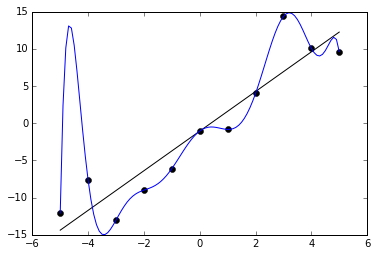
\includegraphics[scale=0.6]{assets/overfitt.png}
    \caption{Overfitting hypothesis}
\end{figure}

You can see that the prediction line fits each data point perfectly, but completely misses out on capturing the relationship between $x$ and $y$ properly.
And now, if we add some brand new data points to the dataset, we see that the predictions on those new examples are way off.

\begin{figure}[!h]
    \centering
    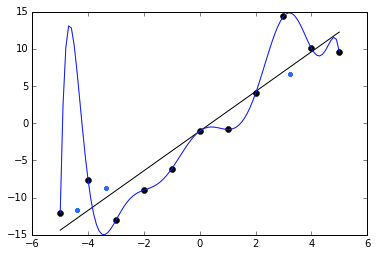
\includegraphics[scale=0.6]{assets/overfitt_with_dots.png}
    \caption{Generalization errors resulting from overfitting}
\end{figure}
This situation is called overfitting, because the model is doing an excessively good job at fitting the data.
It is literally bending over backward to account for the data's mini details.
But most of the data's irregularities are just noise, and they should in fact be ignored.
So because the model overfits, it can't generalize to new data.

% ============================================== %
\section*{Interlude - The training set, the test set, and the happy data scientist}
% ---------------------------------------------- %
To be able to detect overfitting, \textbf{you should always evaluate your model on new data}.\\
\\
New data means, data that your model hasn't seen during training.\\
\\
It's the only way to make sure your model isn't \textit{recalling}.
To do so, now and forever, you must always divide your dataset in (at least) two parts: one for the training, and one for the evaluation of your model.
\newpage
\turnindir{ex09}
\exnumber{09}
\exfiles{data\_spliter.py}
\exforbidden{sklearn}
\makeheaderfilesforbidden


% ================================= %
\section*{Objective}
% --------------------------------- %
Learn how to split a dataset into a \textbf{training set} and a \textbf{test set}.

% ================================= %
\section*{Instructions}
% --------------------------------- %
You must implement a function that \textbf{shuffles} and \textbf{splits} a dataset it in two parts: a \textbf{training set} and a \textbf{test set}.
\begin{itemize}
  \item Your function will shuffle and split the $X$ matrix while keeping a certain \textbf{proportion} of the examples for training, and the rest for testing.
  \item Your function will also shuffle and split the $y$ vector while making sure that the order of the rows in the output match the order of the rows in the split $X$ output.
\end{itemize}


In the \texttt{data\_spliter.py} file create the following function as per the instructions given below:

\begin{minted}[bgcolor=darcula-back,formatcom=\color{lightgrey},fontsize=\scriptsize]{python}
def data_spliter(x, y, proportion):
    """Shuffles and splits the dataset (given by x and y) into a training and a test set,
      while respecting the given proportion of examples to be kept in the training set.
    Args:
      x: has to be an numpy.array, a matrix of dimension m * n.
      y: has to be an numpy.array, a vector of dimension m * 1.
      proportion: has to be a float, the proportion of the dataset that will be assigned to the
        training set.
    Return:
      (x_train, x_test, y_train, y_test) as a tuple of numpy.array
      None if x or y is an empty numpy.array.
      None if x and y do not share compatible dimensions.
      None if x, y or proportion is not of expected type.
    Raises:
      This function should not raise any Exception.
    """
    ... Your code ...
\end{minted}

\warn{
  \begin{itemize}
    \item The dataset has to be randomly shuffled \textit{before} it is split into training and test sets.
    \item Unless you use the same seed in your randomization algorithm, you won't get the same results twice.
  \end{itemize}
}

% ================================= %
\section*{Examples}
% --------------------------------- %
The following examples are just an indication of possible outputs. As long as you have shuffled datasets with their corresponding y values, your function is working correctly.

\begin{minted}[bgcolor=darcula-back,formatcom=\color{lightgrey},fontsize=\scriptsize]{python}
import numpy as np
x1 = np.array([1, 42, 300, 10, 59]).reshape((-1, 1))
y = np.array([0, 1, 0, 1, 0]).reshape((-1, 1))

# Example 1:
data_spliter(x1, y, 0.8)
# Output:
(array([  1,  59,  42, 300]), array([10]), array([0, 0, 1, 0]), array([1]))

# Example 2:
data_spliter(x1, y, 0.5)
# Output:
(array([59, 10]), array([  1, 300,  42]), array([0, 1]), array([0, 0, 1]))

x2 = np.array([[  1, 42],
               [300, 10],
               [ 59,  1],
               [300, 59],
               [ 10, 42]])
y = np.array([0, 1, 0, 1, 0]).reshape((-1, 1))

# Example 3:
data_spliter(x2, y, 0.8)
# Output:
(array([[ 10,  42],
        [300,  59],
        [ 59,   1],
        [300,  10]]),
 array([[ 1, 42]]),
 array([0, 1, 0, 1]),
 array([0]))

# Example 4:
data_spliter(x2, y, 0.5)
# Output:
(array([[59,  1],
        [10, 42]]),
 array([[300,  10],
        [300,  59],
        [  1,  42]]),
 array([0, 0]),
 array([1, 1, 0]))
\end{minted}


% ===========================(fin ex 09)         %
% ============================================== %

\newpage

% ============================================== %
% ===========================(start ex 10)       %
\chapter{Exercise 10}
\extitle{Machine Learning for Grown-ups: Trantor guacamole business}
\turnindir{ex10}
\exnumber{10}
\exfiles{space\_avocado.py, benchmark\_train.py,  models.[csv/yml/pickle]}
\exforbidden{sklearn}
\makeheaderfilesforbidden


% ================================= %
\section*{Objective}
% --------------------------------- %
Let's do Machine Learning for "real"!

% ================================= %
\section*{Introduction}
% --------------------------------- %
The dataset is constituted of 5 columns:
\begin{itemize}
  \item \textbf{index}: not relevant,
  \item \textbf{weight}: the avocado weight order (in ton),
  \item \textbf{prod\_distance}: distance from where the avocado ordered is produced (in Mkm),
  \item \textbf{time\_delivery}: time between the order and the receipt (in days),
  \item \textbf{target}: price of the order (in trantorian unit).
\end{itemize}
It contains the data of all the avocado purchase made by Trantor administration (guacamole is a serious business there).

% ================================= %
\section*{Instructions}
% --------------------------------- %
You have to explore different models and select the best you find.
To do this:
\begin{itemize}
  \item Split your \texttt{space\_avocado.csv} dataset into a training and a test set.
  \item Use your \texttt{polynomial\_features} method on your training set.
  \item Consider several Linear Regression models with polynomial hypothesis with a maximum degree of 4.
  \item Evaluate your models on the test set.
\end{itemize}

According to your model evaluations, what is the best hypothesis you can get?
\begin{itemize}
  \item Plot the evaluation curve which help you to select the best model (evaluation metrics vs models).
  \item Plot the true price and the predicted price obtain via your best model (3D representation or 3 scatterplots).
\end{itemize}


The training of all your models can take a long time.
Thus you need to train only the best one during the correction.
But, you should return in \texttt{benchmark\_train.py} the program which perform the training of all the models and save the parameters of the different models into a file.
In \texttt{models.[csv/yml/pickle]} one must find the parameters of all the models you have explored and trained.
In \texttt{space\_avocado.py} train the model based on the best hypothesis you find and load the other models from \texttt{models.[csv/yml/pickle]}.
Then evaluate and plot the different graphics as asked before.

% ===========================(fin ex 10)         %
% ============================================== %

\newpage

% ============================================== %
% ===========================(start ex 11)       %
\chapter{Conclusion - What you have learned}

The excercises serie is finished, well done!
Based on all the knowledges tackled today, you should be able to discuss and answer the following questions:

\begin{enumerate}
  \item What is the main (obvious) difference between univariate and multivariate linear regression?
  \item Is there a minimum number of variables needed to perform a multivariate linear regression?
  \item Is there a maximum number of variables needed to perform a multivariate linear regression?
        In theory and in practice?
  \item Is there a difference between univariate and multivariate linear regression in terms of performance evaluation?
  \item What does it mean geometrically to perform a multivariate gradient descent with two variables?
  \item Can you explain what is overfitting?
  \item Can you explain what is underfitting?
  \item Why is it important to split the data set in a training and a test set?
  \item If a model overfits, what will happen when you compare its performance on the training set and the test set?
  \item If a model underfits, what do you think will happen when you compare its performance on the training set and the test set?
\end{enumerate}

% ===========================(fin ex 11)         %
% ============================================== %

\newpage

% ================================= %
\section*{Contact}
% --------------------------------- %
You can contact 42AI association by email: contact@42ai.fr\\
You can join the association on \href{https://join.slack.com/t/42-ai/shared_invite/zt-ebccw5r7-YPkDM6xOiYRPjqJXkrKgcA}{42AI slack}
and/or posutale to \href{https://forms.gle/VAFuREWaLmaqZw2D8}{one of the association teams}.

% ================================= %
\section*{Acknowledgements}
% --------------------------------- %
The modules Python \& ML is the result of a collective work, we would like to thanks:
\begin{itemize}
  \item Maxime Choulika (cmaxime),
  \item Pierre Peigné (ppeigne),
  \item Matthieu David (mdavid).
\end{itemize}
who supervised the creation, the enhancement and this present transcription.

\begin{itemize}
  \item Amric Trudel (amric@42ai.fr)
  \item Benjamin Carlier (bcarlier@student.42.fr)
  \item Pablo Clement (pclement@student.42.fr)
\end{itemize}
for your investment for the creation and development of these modules.

\begin{itemize}
  \item Richard Blanc (riblanc@student.42.fr)
  \item Solveig Gaydon Ohl (sgaydon-@student.42.fr)
  \item Quentin Feuillade Montixi (qfeuilla@student.42.fr)
\end{itemize}
who betatest the first version of the modules of Machine Learning.
\vfill
\doclicenseThis

\end{document}
